\documentclass[Rapport/Rapport_main.tex]{subfiles}
\begin{document}
\subsection{Cup Light}\label{sec:rap_cup_light}
I dette afsnit beskrives de designvalg, der er gjort angående lyset i en CupHolder og controlleren dertil, samt hvordan de er implementeret. Til sidst laves der også en test for modulet. Dette modul anvendes udelukkende af GameController-klassen på PSoC playerside.
\subsubsection{Hardwaredesign}
\textbf{Lys på CupHolder}\\
Den overordnede hardware for koppen kan deles op i 2 dele. En del der hører til på Cup Holder, og et controller-kredsløb der anvendes til at styre lyset, og som befinder sig på Cup Holder Controller.\\
På Cup Holder er det fysiske lys placeret. Det fysiske lys må ikke fylde meget og heller ikke være dyrt, da det skal passe i forhold til antallet af lys på og målene for en Cup Holder, der kan ses i bilag \textbf{Kravspecifikation} i afsnit \fullref{kravspec:sec:ikke_funktionelle_krav}. Det besluttes derfor, at der anvendes en common-cathode RGB-led med en diameter på 5mm \cite{RGBledDatasheet}. Der vælges almindelige RGB-LED'er over fx addresserbare RGB-led'er pga. prisen, da der ikke er et krav om, at de enkelte LED'er på hver kopholder skal kunne lyse individuelt.\\
RGB-LED'erne skal have formodstande til de ben, der anvendes til at styre farverne. Formodstandene afhænger af diodespændingen, hvilket giver forskellige værdier. Der skal også være 3 transistorer\cite{datasheet_bc557b} til at tænde for benene efter behov. Designet af lyset på Cup Holder kan ses i figur \ref{fig:rap_cupholder_light}.
\begin{figure}[H]
    \centering
    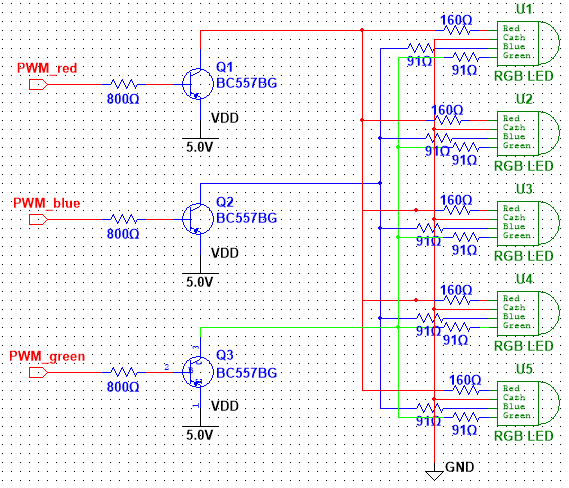
\includegraphics[width=0.9\textwidth]{HardwareDesign/CupLight/graphics/CupHolder_HW.png}
    \caption{Design af CupLight på Cupholder}
    \label{fig:rap_cupholder_light}
\end{figure}
\textbf{Controller-kredsløb til Cup Light}\\
Kredsløbet der skal kontrollere lyset i Cup Holders, skal kunne lave PWM-signaler nok til alle Cup Holders. Der skal altså laves 18 PWM-signaler, da den røde, grønne og blå farve skal kunne kontrolleres på alle 6 Cup Holders.\\
Cup Light Controller-kredsløbet laves af 3 74HC595 skifteregistre\cite{datasheet_shiftreg}, hvor der kan laves et PWM-signal på deres output ben ved at styre registrene gennem SPI-kommunikation. På denne måde er man med 3 registre i stand til at lave 24 individuelle PWM-signaler. De kan så forbindes til de forskellige transistorer i CupHolders. Designet af CupLight controlleren kan ses i figur \ref{fig:rap_cuplight_controller}.
\begin{figure}[H]
    \centering
    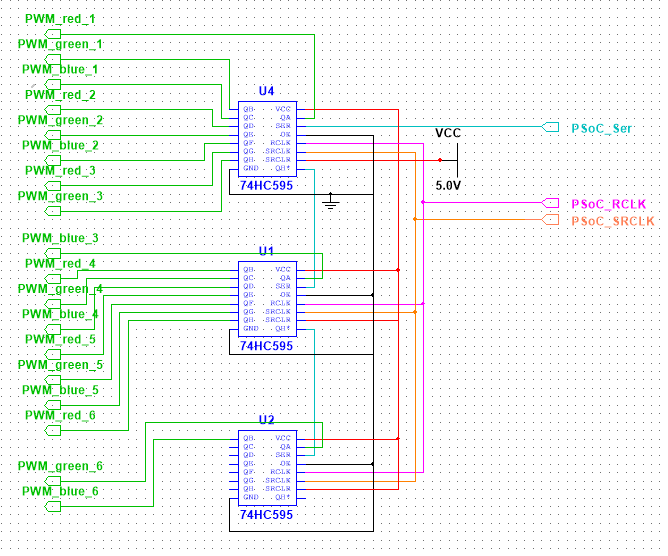
\includegraphics[width=0.9\textwidth]{HardwareDesign/CupLight/graphics/CupLight_HW_Controller.png}
    \caption{Design af controller for CupLight}
    \label{fig:rap_cuplight_controller}
\end{figure}
Hardwaredesignet er videre udspecificeret i dokumentet \textbf{Hardware Design} i afsnit \fullref{hwdesign:sec:cuplight_hw_design}.
\subsubsection{Softwaredesign}
Der skal laves kode til at styre CupLight controller hardwaren. Det vil sige, at der skal laves software, der ved SPI-kommunikation kontrollerer et skifteregister til at outputte det ønskede PWM-signal på et output pin. Til dette kan der anvendes et timer-interrupt, der bestemmer, hvornår skifteregisteret skal opdateres med nye værdier. Der laves desuden et klassediagram for dette interface, der kan ses på figur \ref{fig:rap_cd_cuplight}.
\begin{figure}[H]
    \centering
    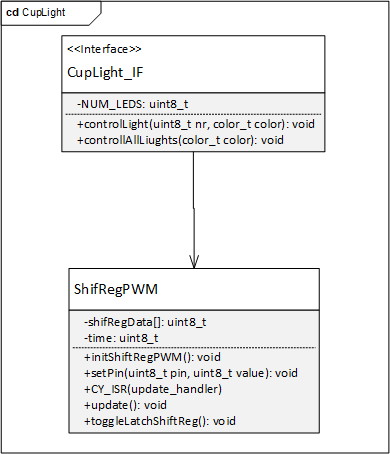
\includegraphics[width=0.5\textwidth]{Softwaredesign/CupLight_IF/graphics/CD_CupLight.png}
    \caption{Klassediagram for CupLight modulet}
    \label{fig:rap_cd_cuplight}
\end{figure}
Alt Software design er udspecificeret mere i \textbf{Software Design} bilaget i afsnit \fullref{swdesign:sec:cuplight_sw_design}.
\subsubsection{Implementering}
Implementeringen af CupLight\_IF er lavet i IDE'et PSoC-creator 4.2. Det er implementeret ved moduler bestående af header- og source-filer. Til implementeringen af \textsc{ShiftRegPWM} er der hentet inspiration\cite{shiftregpwm}. De vigtigste funktioner og detaljer i implementeringen kan ses i bilaget \textbf{Softwaredesign} i afsnit \fullref{swdesign:sec:cuplight_sw_impl}.
\subsubsection{Modultest}
Til test af CupLight modulet anvendes et UART-komponent på PSoC'en til at sætte forskellige PWM-værdier. PSoC'ens SPI-kommunikation forbindes til et 74HC595 skifteregister, og på output pins af dette register måles forskellige PWM-signaler. Der blev målt rise-time af PWM-signalet, samt nøjagtigheden af PWM-signalet. Senere forbindes controller-kredsløbet til en LED for at teste, at farverne stemmer overens med hvad forventes. Forskellige pins på controlleren testes for at tjekke, om LED'er kan styres individuelt, som det angives af \textbf{Kravspecifikationen} i afsnit \fullref{kravspec:sec:ikke_funktionelle_krav}. Samtlige resultater fra modultesten kan ses i dokumentet \textbf{Modultest} i afsnit \fullref{modultest:sec:cuplight_test}.\\\\
Konklusionen af modultesten er, at controller modulet er i stand til at generere tilstrækkeligt præcise PWM-signaler til at kunne styre RGB-led'er til mere end 10 forskellige farver. 
\end{document}